\documentclass[a4, 12pt, footinclude=true, headinclude=true, oneside]{article}


\usepackage{hyperref}
\usepackage{tikz}
	 \usetikzlibrary{%
		decorations.fractals%
		,decorations.pathmorphing%
		,shadows%
	}
\usepackage[top=2cm, left=2cm, bottom=2cm, right=2cm]{geometry}	
\usepackage{MnSymbol}

\setlength{\parindent}{0pt}

\author{Jokobus}
\title{TikZ pictures}

\begin{document}
	\maketitle
	This \LaTeX document contains some random, but beautiful TikZ plots. Feel free to use and modify them for your personal use. 
	
	\vspace*{2cm}
	
	\begin{figure}[h]
		\centering
		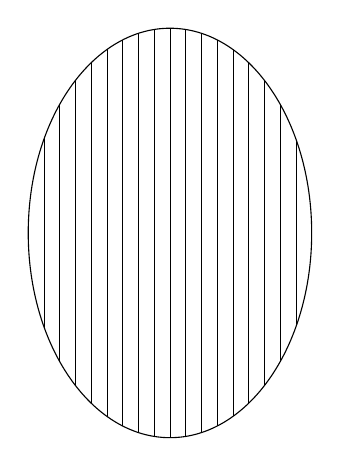
\begin{tikzpicture}[scale=2]
			\clip[draw] (0,0) ellipse [x radius=0.9cm, y radius=1.3cm];
			\foreach \x in {-0.8, -0.7,...,0.9} {
				\draw[step=.5cm, very thin] (\x,2) -- (\x,-2);
			}
		\end{tikzpicture}
		\caption{Picture of a monochrome Easter egg}
	\end{figure}
	 	
	 \begin{figure}[h]
	 	\centering
	 	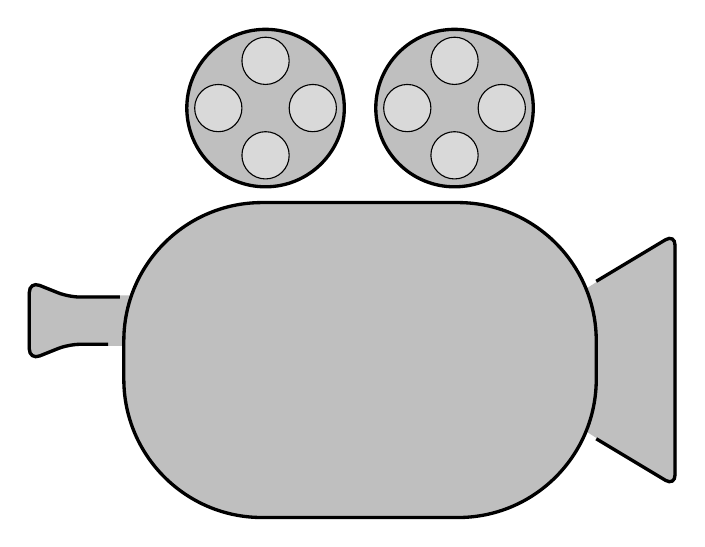
\begin{tikzpicture}
			\draw[fill=lightgray, very thick] (-1.2,3.2) circle (1cm);
			\draw[fill=lightgray!60!white] (-1.2,2.6) circle (0.3cm);
			\draw[fill=lightgray!60!white] (-0.6,3.2) circle (0.3cm);
			\draw[fill=lightgray!60!white] (-1.2,3.8) circle (0.3cm);
			\draw[fill=lightgray!60!white] (-1.8,3.2) circle (0.3cm);
			
			\draw[fill=lightgray, very thick] (1.2,3.2) circle (1cm);
			\draw[fill=lightgray!60!white] (1.2,2.6) circle (0.3cm);
			\draw[fill=lightgray!60!white] (0.6,3.2) circle (0.3cm);
			\draw[fill=lightgray!60!white] (1.2,3.8) circle (0.3cm);
			\draw[fill=lightgray!60!white] (1.8,3.2) circle (0.3cm);
			
			\filldraw[lightgray,very thick, rounded corners] (2.9,0.9) -- (4,1.6) -- (4,-1.6) -- (2.9,-0.9);
			\draw[very thick, rounded corners] (3,1) -- (4,1.6) -- (4,-1.6) -- (3,-1);
			
			\filldraw[lightgray, very thick, rounded corners] (-2.8,0.8) -- (-3.7,0.8) -- (-4.2,1) -- (-4.2,0) -- (-3.7,0.2) -- (-2.9,0.2);
			\draw[very thick, rounded corners] (-3.05,0.8) -- (-3.7,0.8) -- (-4.2,1) -- (-4.2,0) -- (-3.7,0.2) -- (-3.2,0.2);
			
			\filldraw[fill=lightgray, very thick, rounded corners=50] (-3,2) rectangle (3,-2);
		\end{tikzpicture}
		\caption{Taken by a monochrome camera}
	\end{figure}
	
	\begin{figure}[h]
		\centering
		\begin{tikzpicture}
			\draw[black][<-] (-2.5,5) -- (-2.5,0);
			\draw[black] (-2.5,0) -- (2.5,0);
			\draw[black][<-] (2.5,0) -- (2.5,5);

			\draw[red] (-2.5,1) -- (2.5,1);
			\draw[red] (-2.5,2.5) -- (2.5,2.5);
			\draw[red] (-2.5,4.5) -- (2.5,4.5);
			\filldraw (2.5,1) circle (0pt) node[anchor=west]{$E_1$};
			\filldraw (2.5,2.5) circle (0pt) node[anchor=west]{$E_2$};
			\filldraw (2.5,4.5) circle (0pt) node[anchor=west]{$E_3$};
		\end{tikzpicture}
	\caption{Der Potentialtopf mit unendlich hohen Wänden}
	\end{figure}


	\begin{figure}[h]
		\centering
		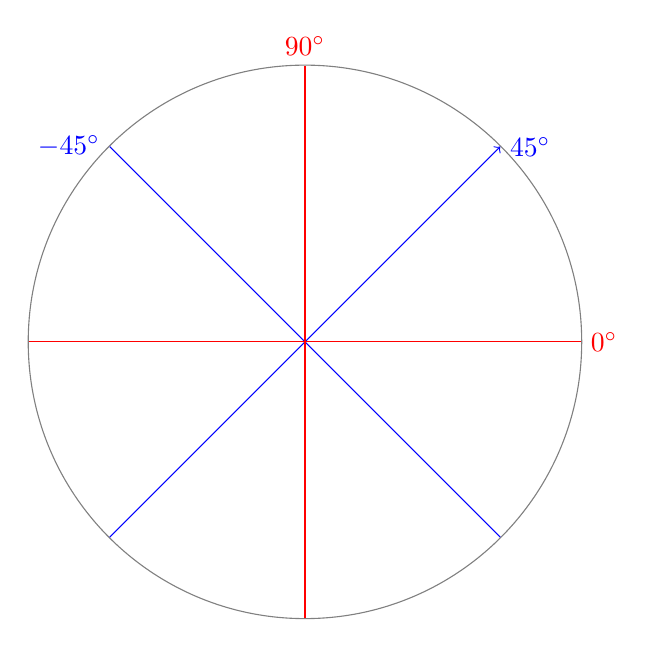
\begin{tikzpicture}
			\draw[gray] circle (100pt);
			\draw[blue][->] (-2.48,-2.48) -- (2.48,2.48) node[anchor=west]{$45^\circ$};
			\draw[blue] (2.48,-2.48) -- (-2.48,2.48)node[anchor=east]{$-45^\circ$};
			\draw[red] (-3.507,0) -- (3.507,0)node[anchor=west]{$0^\circ$};
			\draw[red] (0,-3.507) -- (0,3.507) node[anchor=south]{$90^\circ$};
			
		\end{tikzpicture}
		\caption{Circle with degrees}
	\end{figure}

	\begin{figure}[h]
		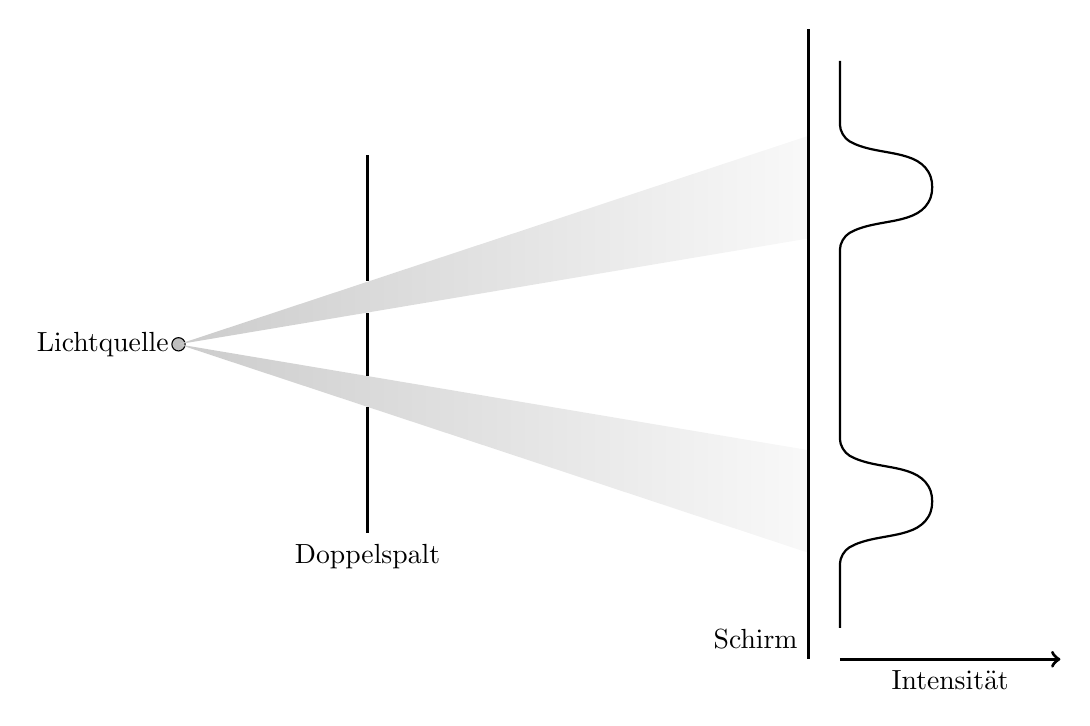
\begin{tikzpicture}[scale=0.8]
			\draw[fill=lightgray] (0,0) circle (3pt);
			\node[left]{Lichtquelle};	
			%	\draw [gray] (0.25,-0.28) arc [radius=0.5, start angle=-45, end angle=45]; 
			\shade[left color=lightgray!80, right color=lightgray!10] (0,0) -- (10,3.31) -- (10,1.68);
		%	\draw[dashed] (0,0) -- (10,3.31);
			%\draw[thin, fill=lightgray] (0,0) -- (10,3.31) -- (10,1.68);
		%	\draw [dashed](0,0) -- (10,1.68);
			\shade[left color=lightgray!80, right color=lightgray!10] (0,0) -- (10,-3.31) -- (10,-1.68); 
			
		%	\draw[dashed] (0,0) -- (10,-1.68);
		%	\draw[dashed] (0,0) -- (10,-3.31);
			
			\draw[very thick] (3,3) -- (3,1);
			\draw[very thick] (3,0.5) -- (3,-0.5);
			\draw[very thick] (3,-1) -- (3,-3) node[below]{Doppelspalt};
			
			
			%\draw[->, rounded corners, very thick](10,6) -- (10,-6)node[above left]{Schirm} -- (10.5,-5.5)-- node[below]{Intensität} (14,-5.5);
			\draw[very thick](10,5) -- (10,-5)node[above left]{Schirm};
			\draw[->, very thick] (10.5,-5)-- node[below]{Intensität} (14,-5);
			
		%	\draw [rounded corners](10.5,3.31) to [out=330,in=110] (12,2.495) to [out=250,in=30] (10.5,1.68);
		%%	\draw [rounded corners](10.5,-1.68) to [out=330,in=105] (12,-2.495) to [out=270,in=30] (10.5,-3.31);
			\draw[rounded corners, thick](10.5,4.5) to [out=270,in=90](10.5,3.31) to [out=330,in=110] (12,2.495) to [out=250,in=30] (10.5,1.68) to [out=270, in= 90] (10.5,-1.68) to [out=330,in=110] (12,-2.495) to [out=250,in=30] (10.5,-3.31) to[out=270,in=90](10.5,-4.5) ;
	
			%\draw[rounded corners](10.5,5) to (10.5,3.31) to (12,2.495) to (10.5,1.68) to (10.5,-1.68) to (12,-2.495) to (10.5,-3.31) to (10.5,-5) ;
			
			%\draw[->] (10.5,-5.5)--node[below]{Intensität} (15,-5.5);
		\end{tikzpicture}
		\caption{Doppelspalt - Teilchencharakter}
	\end{figure}

	\begin{figure}[h]
		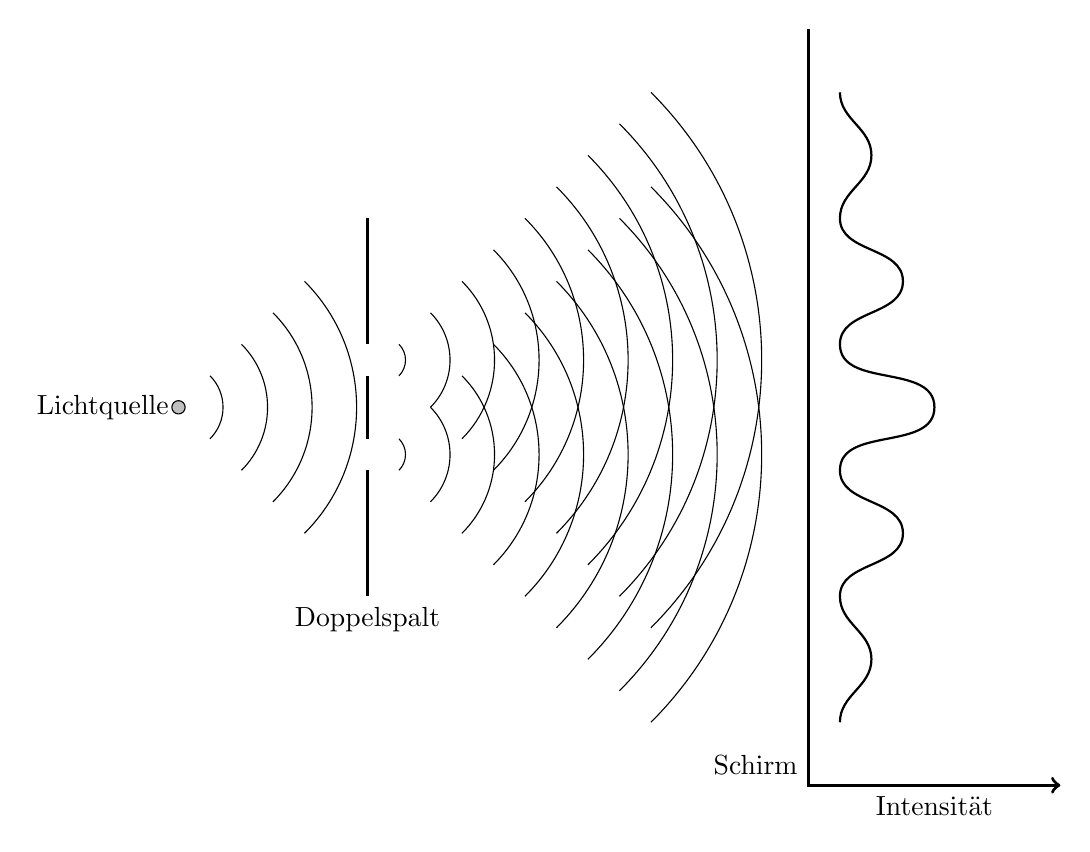
\begin{tikzpicture}[scale=0.8]
			\draw[fill=lightgray] (0,0) circle (3pt);
			\node[left]{Lichtquelle};	
			%	\draw [gray] (0.25,-0.28) arc [radius=0.5, start angle=-45, end angle=45]; 
			\draw (.5,.5) to[out=-45, in=45] (.5,-.5);
			\draw (1,1) to[out=-45, in=45] (1,-1);
			\draw (1.5,1.5) to[out=-45, in=45] (1.5,-1.5);
			\draw (2,2) to[out=-45, in=45] (2,-2);
			
			
			\draw[very thick] (3,3) -- (3,1);
			\draw[very thick] (3,0.5) -- (3,-0.5);
			\draw[very thick] (3,-1) -- (3,-3) node[below]{Doppelspalt};
			
			
			\foreach \x in {0,0.5,...,4} {
				\draw (3.5+\x,1+\x) to[out=-45, in=45] (3.5+\x,.5-\x);
			}
			\foreach \x in {0,0.5,...,4} {
				\draw (3.5+\x,-1-\x) to[out=45, in=-45] (3.5+\x,-.5+\x);
			}
			
			%\draw[->, rounded corners, very thick](10,6) -- (10,-6)node[above left]{Schirm} -- (10.5,-5.5)-- node[below]{Intensität} (14,-5.5);
			\draw[->, very thick](10,6) -- (10,-6)node[above left]{Schirm} -- node[below]{Intensität} (14,-6);
			\draw[thick] (10.5,5) to [out=270,in=90](11,4) to [out=270,in=90](10.5,3) to [out=270,in=90](11.5,2) to[out=270,in=90](10.5,1) to [out=270,in=90](12,0) to [out=270,in=90](10.5,-1) to [out=270,in=90](11.5,-2) to [out=270,in=90](10.5,-3) to [out=270,in=90] (11,-4) to [out=270,in=90](10.5,-5);
			%\draw[->] (10.5,-5.5)--node[below]{Intensität} (15,-5.5);
		\end{tikzpicture}
			\caption{Doppelspalt - Wellencharakter}
	\end{figure}
 	
 	\begin{figure}[h]
 		\centering
 		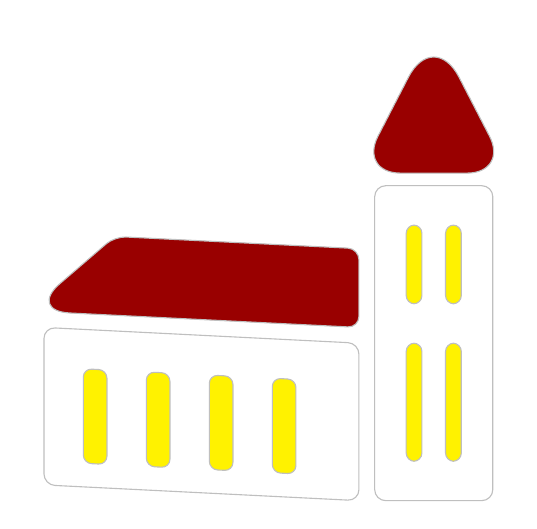
\begin{tikzpicture}
	 		% church
	 		\filldraw[fill=white, draw=lightgray, rounded corners, yslant=-0.05] (-6,10.4) rectangle (-2,8.4);
	 		% roof
	 		\filldraw[fill=red!60!black, draw=lightgray, rounded corners, yslant=-0.05] (-5.1,11.6) to [rounded corners= 15] (-6.2,10.6) -- (-2,10.6) -- (-2,11.6) -- cycle;
	 		% tower
	 		\filldraw[fill=white, draw=lightgray, rounded corners] (-1.8,12.5) rectangle (-0.3,8.5);
	 		% roof of the tower
	 		\filldraw[fill=red!60!black, draw=lightgray, rounded corners=15] (-2,12.66) -- (-0.1,12.66) to [rounded corners= 20] (-1.05,14.5) -- cycle;
	 		% windows
	 		\draw[fill=yellow, draw=lightgray, rounded corners=3, yslant=-0.05] (-5.5,9.9) rectangle (-5.2,8.7);
	 		\draw[fill=yellow, draw=lightgray, rounded corners=3, yslant=-0.05] (-4.7,9.9) rectangle (-4.4,8.7);
	 		\draw[fill=yellow, draw=lightgray, rounded corners=3, yslant=-0.05] (-3.9,9.9) rectangle (-3.6,8.7);
	 		\draw[fill=yellow, draw=lightgray, rounded corners=3, yslant=-0.05] (-3.1,9.9) rectangle (-2.8,8.7);
	 		% bottom winodws of the tower
	 		\draw[fill=yellow, draw=lightgray, rounded corners=3] (-1.4,10.5) rectangle (-1.2,9);
	 		\draw[fill=yellow, draw=lightgray, rounded corners=3] (-0.7,10.5) rectangle (-0.9,9);
	 		% upper windows of the tower
	 		\draw[fill=yellow, draw=lightgray, rounded corners=3] (-1.4,12) rectangle (-1.2,11);
	 		\draw[fill=yellow, draw=lightgray, rounded corners=3] (-0.7,12) rectangle (-0.9, 11);
 		\end{tikzpicture}
 		\caption{Modern church}
 	\end{figure}

	\begin{figure}[h]
		\centering
		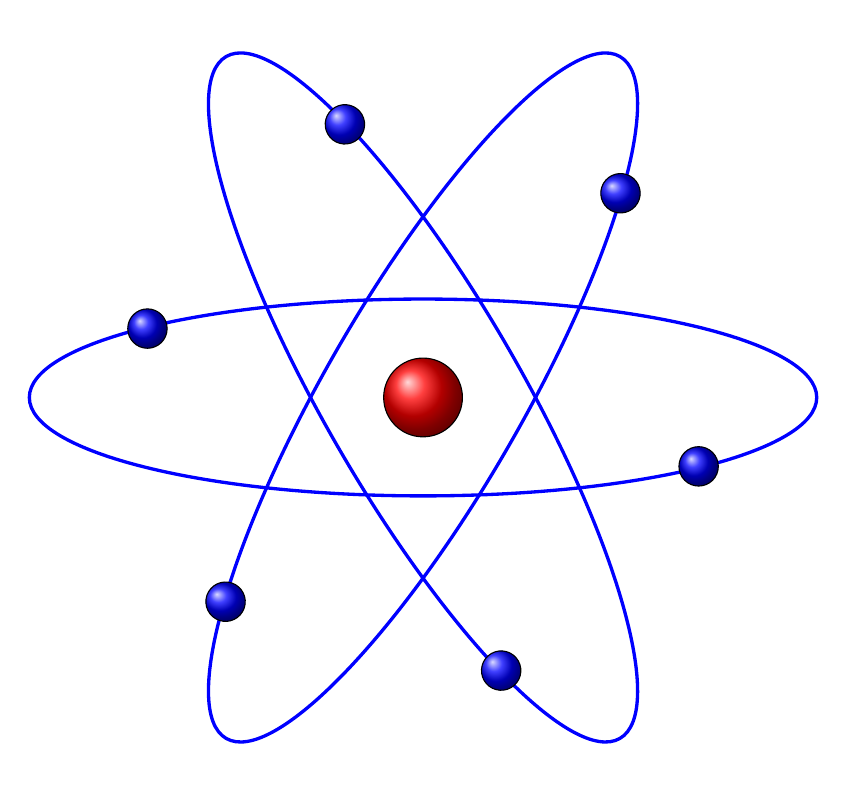
\begin{tikzpicture}[scale=0.5]
			% Nucleus
			\shadedraw[shading=ball, ball color=red] (0,0) circle (1cm);
			
			% Electrons
			\foreach \x in {0, 1, 2}	{	
				\draw[rotate= 60*\x, blue, very thick] (0,0) ellipse [x radius=10cm, y radius=2.5cm];
				\shadedraw[shading=ball, fill=blue!80!black, rotate around={60*\x:(0,0)}] (-7,1.75) circle (0.5cm);
				\shadedraw[shading=ball, fill=blue!80!black, rotate around={60*\x:(0,0)}] (7,-1.75) circle (0.5cm);		
			}		
		\end{tikzpicture}
			\caption{Rutherford}
	\end{figure}
	
	\pagebreak
	\begin{figure}[h!]
		\centering
		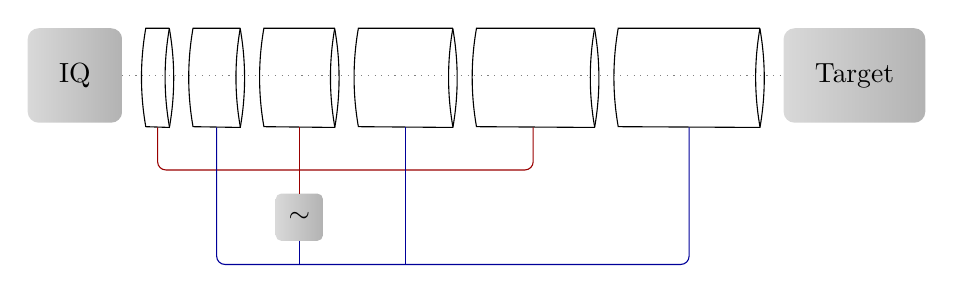
\begin{tikzpicture}[scale=1.2]
			\shade[left color=gray!30, right color=gray!60, rounded corners=4] (0,0.5)rectangle (-1,-0.5);
			\node at (-0.5,0){IQ};
			\draw[gray, dotted] (0,0) -- (7,0);
			
			
			\shade[left color=gray!30, right color=gray!60, rounded corners=4] (7,0.5) rectangle (8.5,-0.5);
			\node at (7.75,0){Target};
			
			% First
			\draw (0.5,0.5) arc [start angle=170, end angle=190, radius=3cm];
			\draw (0.5,0.5) -- (0.25,0.5) arc [start angle=170, end angle=190, radius=3cm] -- (0.5,-0.55) arc [gray, start angle=-10, end angle=10, radius=3cm]; 
			
			% Second
			\draw (1.25,0.5) arc [start angle=170, end angle=190, radius=3cm];
			\draw (1.25,0.5) -- (0.75,0.5) arc [start angle=170, end angle=190, radius=3cm] -- (1.25,-0.55) arc [gray, start angle=-10, end angle=10, radius=3cm]; 
			
			% Third
			\draw (2.25,0.5) arc [start angle=170, end angle=190, radius=3cm];
			\draw (2.25,0.5) -- (1.5,0.5) arc [start angle=170, end angle=190, radius=3cm] -- (2.25,-0.55) arc [gray, start angle=-10, end angle=10, radius=3cm]; 
			
			% Fourth
			\draw (3.5,0.5) arc [start angle=170, end angle=190, radius=3cm];
			\draw (3.5,0.5) -- (2.5,0.5) arc [start angle=170, end angle=190, radius=3cm] -- (3.5,-0.55) arc [gray, start angle=-10, end angle=10, radius=3cm]; 
			
			% Sixth
			\draw (5,0.5) arc [start angle=170, end angle=190, radius=3cm];
			\draw (5,0.5) -- (3.75,0.5) arc [start angle=170, end angle=190, radius=3cm] -- (5,-0.55) arc [gray, start angle=-10, end angle=10, radius=3cm]; 
			
			% Seventh
			\draw (6.75,0.5) arc [start angle=170, end angle=190, radius=3cm];
			\draw (6.75,0.5) -- (5.25,0.5) arc [start angle=170, end angle=190, radius=3cm] -- (6.75,-0.55) arc [gray, start angle=-10, end angle=10, radius=3cm]; 
			
			
			% DC
			\shade[left color=gray!30, right color=gray!60, rounded corners=2] (1.625,-1.25) rectangle (2.125,-1.75);
			\node at (1.875,-1.5){$\sim$};
			
			% DC 1
			\draw[red!60!black, rounded corners=3] (0.375,-0.55) -- (0.375,-1) -- (4.35,-1) -- (4.35,-0.55);
			\draw[red!60!black] (1.875,-0.55) -- (1.875,-1.25);
			
			% DC 2
			\draw[blue!60!black, rounded corners=3] (1,-0.55) -- (1,-2) -- (6,-2) -- (6,-0.55);
			\draw[blue!60!black] (3,-0.55) -- (3,-2);
			\draw[blue!60!black] (1.875,-1.75) -- (1.875,-2);
		\end{tikzpicture}	
		\caption{Linearbeschleuniger}
	\end{figure}
	
	\begin{figure}[h!]
		\centering
		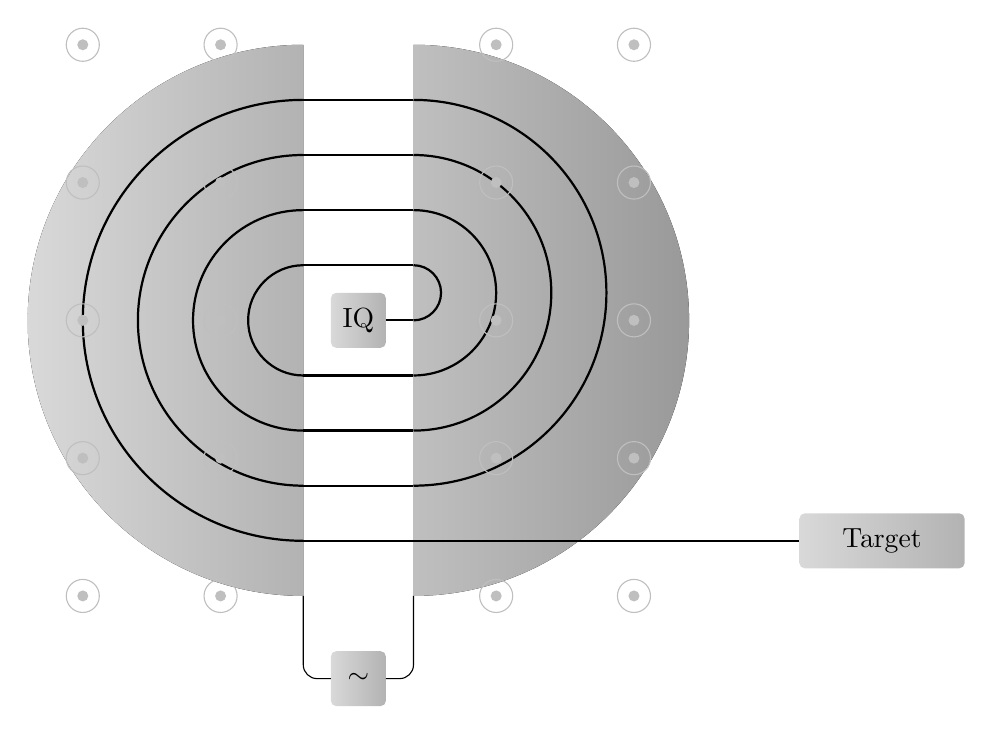
\begin{tikzpicture}[scale=0.7]
			\centering
			% Left Duant
			\fill[left color=gray!30, right color=gray!60] (-1,-5) -- (-1,5) arc [start angle=90, end angle=270, x radius=5cm, y radius=5cm];
			
			% Right Duant
			\fill[left color=gray!50, right color=gray!80] (1,5) -- (1,-5) arc [start angle=-90, end angle=90, x radius=5cm, y radius=5cm];
			
			% Target
			\shade[left color=gray!30, right color=gray!60, rounded corners=2] (8,-3.5) rectangle (11,-4.5);
			\node at (9	.5,-4){Target};
			
			% Source
			\shade[left color=gray!30, right color=gray!60, rounded corners=2] (-0.5,-0.5) rectangle (0.5,0.5);
			\node at (0,0){IQ};
			
			% DC
			\shade[left color=gray!30, right color=gray!60, rounded corners=2] (-0.5,-6) rectangle (0.5,-7);
			\node at (0,-6.5){$\sim$};
			\draw[rounded corners=5] (-0.5,-6.5) -- (-1,-6.5) -- (-1,-5);
			\draw[rounded corners=5] (0.5,-6.5) -- (1,-6.5) -- (1,-5);
			
			% Source to RD
			\draw[thick] (0.5,0) -- (1,0);
			
			% R 1
			\draw[thick] (1,0) arc [start angle=-90, end angle=90, radius=0.5];
			\draw[thick] (1,1) -- (-1,1);
			
			% L 1
			\draw[thick] (-1,1) arc [start angle=90, end angle=270, radius=1];
			\draw[thick] (1,-1) -- (-1,-1);
			
			% R 2
			\draw[thick] (1,-1) arc [start angle=-90, end angle=90, radius=1.5];
			\draw[thick] (1,2) -- (-1,2);
			
			% L 2
			\draw[thick] (-1,2) arc [start angle=90, end angle=270, radius=2];
			\draw[thick] (1,-2) -- (-1,-2);
			
			% R 3
			\draw[thick] (1,-2) arc [start angle=-90, end angle=90, radius=2.5];
			\draw[thick] (1,3) -- (-1,3);
			
			% L 3
			\draw[thick] (-1,3) arc [start angle=90, end angle=270, radius=3];
			\draw[thick] (1,-3) -- (-1,-3);
			
			% R 4
			\draw[thick] (1,-3) arc [start angle=-90, end angle=90, radius=3.5];
			\draw[thick] (1,4) -- (-1,4);
			
			% L 4
			\draw[thick] (-1,4) arc [start angle=90, end angle=270, radius=4];
			\draw[thick] (1,-3) -- (-1,-3);
			
			% L 4 to Target
			\draw[thick] (-1,-4) -- (8,-4);
			
			% B Feld
			% First
			\draw[lightgray] (-5,5) circle [radius=0.3cm]; \fill[lightgray] (-5,5) circle [radius=0.1];	
			\draw[lightgray] (-5,2.5) circle [radius=0.3cm]; \fill[lightgray] (-5,2.5) circle [radius=0.1];
			\draw[lightgray] (-5,0) circle [radius=0.3cm]; \fill[lightgray] (-5,0) circle [radius=0.1];
			\draw[lightgray] (-5,-2.5) circle [radius=0.3cm]; \fill[lightgray] (-5,-2.5) circle [radius=0.1];
			\draw[lightgray] (-5,-5) circle [radius=0.3cm]; \fill[lightgray] (-5,-5) circle [radius=0.1];	
			
			% Second	
			\draw[lightgray] (-2.5,5) circle [radius=0.3cm]; \fill[lightgray] (-2.5,5) circle [radius=0.1];	
			\draw[lightgray] (-2.5,2.5) circle [radius=0.3cm]; \fill[lightgray] (-2.5,2.5) circle [radius=0.1];
			\draw[lightgray] (-2.5,0) circle [radius=0.3cm]; \fill[lightgray] (-2.5,0) circle [radius=0.1];
			\draw[lightgray] (-2.5,-2.5) circle [radius=0.3cm]; \fill[lightgray] (-2.5,-2.5) circle [radius=0.1];
			\draw[lightgray] (-2.5,-5) circle [radius=0.3cm]; \fill[lightgray] (-2.5,-5) circle [radius=0.1];	
			
			% Fourth
			\draw[lightgray] (2.5,5) circle [radius=0.3cm]; \fill[lightgray] (2.5,5) circle [radius=0.1];	
			\draw[lightgray] (2.5,2.5) circle [radius=0.3cm]; \fill[lightgray] (2.5,2.5) circle [radius=0.1];
			\draw[lightgray] (2.5,0) circle [radius=0.3cm]; \fill[lightgray] (2.5,0) circle [radius=0.1];
			\draw[lightgray] (2.5,-2.5) circle [radius=0.3cm]; \fill[lightgray] (2.5,-2.5) circle [radius=0.1];
			\draw[lightgray] (2.5,-5) circle [radius=0.3cm]; \fill[lightgray] (2.5,-5) circle [radius=0.1];	
			
			% Fifth	
			\draw[lightgray] (5,5) circle [radius=0.3cm]; \fill[lightgray] (5,5) circle [radius=0.1];	
			\draw[lightgray] (5,2.5) circle [radius=0.3cm]; \fill[lightgray] (5,2.5) circle [radius=0.1];
			\draw[lightgray] (5,0) circle [radius=0.3cm]; \fill[lightgray] (5,0) circle [radius=0.1];
			\draw[lightgray] (5,-2.5) circle [radius=0.3cm]; \fill[lightgray] (5,-2.5) circle [radius=0.1];
			\draw[lightgray] (5,-5) circle [radius=0.3cm]; \fill[lightgray] (5,-5) circle [radius=0.1];	
			
		\end{tikzpicture}
		\caption{Zyklotron}
	\end{figure}
	\pagebreak
	\begin{figure}[h!]
		\centering
		
\begin{tikzpicture}[scale=1.2]
			\draw[line width=0.3cm, fill= yellow!60!white](2,0) arc [start angle=0, end angle=180, radius=2cm] to [rounded corners, in=90, out=270](-1,-3) to [rounded corners] (1,-3) to 	[in=270, out=90] cycle;
			\draw[rounded corners, fill=black] (-1, -3.3) rectangle (1, -3.5);
			\draw[rounded corners, fill=black] (-0.8, -3.7) rectangle (0.8, -3.9);
			\draw[rounded corners, fill=black] (-0.6, -4.1) rectangle (0.6, -4.3);	
			
			\draw[line width=0.3cm] (-0.2,-3) -- +(0,2) arc [start angle=0, end angle=270, radius=0.2cm] -- (0.4,-1.2) arc [start angle=-90, end angle=180, radius=0.2cm] -- +(0,-2); 
			
			\foreach \x in {-120, -100, -80, -60, -40, -20, 0, 20, 40, 60, 80, 100, 120}{
				\draw[rounded corners, fill=black, rotate around={\x:(0,0)}] (-0.1,3.5) rectangle (0.1, 2.5);
			}		
			
			\node at (-4,3) {\huge ?};
			\node at (4,-3) {\Huge ?};
			\node at (3,4) {\huge ?};
			\node at (4,2) {\huge ?};
			\node at (-4,-2) {\Large ?};
			\node at (-3,-4) {\Huge ?};
			\node at (-2,4) {\Large ?};	
		\end{tikzpicture}
		\vspace{1cm}
		\caption{There shall be light}
	\end{figure}
 
\end{document}	